
% this file is called up by thesis.tex
% content in this file will be fed into the main document
%----------------------- introduction file header -----------------------
%%%%%%%%%%%%%%%%%%%%%%%%%%%%%%%%%%%%%%%%%%%%%%%%%%%%%%%%%%%%%%%%%%%%%%%%%
%  Capítulo 1: Introducción- DEFINIR OBJETIVOS DE LA TESIS              %
%%%%%%%%%%%%%%%%%%%%%%%%%%%%%%%%%%%%%%%%%%%%%%%%%%%%%%%%%%%%%%%%%%%%%%%%%

\chapter{Planteamiento del problema}

%: ----------------------- HELP: latex document organisation
% the commands below help you to subdivide and organise your thesis
%    \chapter{}       = level 1, top level
%    \section{}       = level 2
%    \subsection{}    = level 3
%    \subsubsection{} = level 4
%%%%%%%%%%%%%%%%%%%%%%%%%%%%%%%%%%%%%%%%%%%%%%%%%%%%%%%%%%%%%%%%%%%%%%%%%
%                           Presentación                                %
%%%%%%%%%%%%%%%%%%%%%%%%%%%%%%%%%%%%%%%%%%%%%%%%%%%%%%%%%%%%%%%%%%%%%%%%%

\section{Definición del problema}


%%%%%%%%%%%%%%%%%%%%%%%%%%%%%%%%%%%%%%%%%%%%%%%%%%%%%%%%%%%%%%%%%%%%%%%%%
%                           Def_ Probelma                                    %
%%%%%%%%%%%%%%%%%%%%%%%%%%%%%%%%%%%%%%%%%%%%%%%%%%%%%%%%%%%%%%%%%%%%%%%%%

En la actualidad la empresa realiza funciones de soporte técnico e inventarios  siendo así una de las vertientes del negocio más importantes, por la exposición directa al cliente, la empresa atraviesa  por dificultades con dichos  aspectos debido a la carencia de un software propio que pueda brindar datos en tiempo real de dichos servicios y que a su vez pueda proporcionar un reporteo claro  con datos duros que de pauta a el análisis y a la solución de los incidentes, dado que se cuenta con un impacto directo al SLA (Service Level Agreement) del 21.5\%  de incumplimiento promedio de tiempos de atención asignado, como se muestra en la tabla \ref{tab:PDP1} y la tabla \ref{tab:PDP2} ,  estos incumplimientos provocan penalizaciones, que se estipulan bajo contrato, con la consecuente pérdida de recursos, afectando directamente la imagen de la empresa, con la consecuente pérdida de contratos.

\begin{table}[htbp]
	\centering
	\caption{Representación del SLA de cumplimiento e incumplimiento de tiempos de servicios requeridos estipulados a nivel contrato, zona foránea}
	\scalebox{0.55}{\begin{tabular}{|c|c|c|c|c|c|c|c|}
			\toprule
			\rowcolor[rgb]{ .188,  .329,  .588} \textcolor[rgb]{ 1,  1,  1}{\textbf{Empresa}} & \textcolor[rgb]{ 1,  1,  1}{\textbf{Total dentro del SLA}} & \textcolor[rgb]{ 1,  1,  1}{\textbf{Total fuera del SLA}} & \textcolor[rgb]{ 1,  1,  1}{\textbf{Total de servicios}} & \textcolor[rgb]{ 1,  1,  1}{\textbf{Porcentual }} & \textcolor[rgb]{ 1,  1,  1}{\textbf{Otras areas}} & \textcolor[rgb]{ 1,  1,  1}{\textbf{Total fuera de SLA}} & \textcolor[rgb]{ 1,  1,  1}{\textbf{Total general}} \\
			\midrule
			\multicolumn{1}{|l|}{Diconsa} & 15 & 26 & 41 & \textcolor[rgb]{ 1,  0,  0}{36.5853659} & 87 & 113 & 128 \\
			\midrule
			\multicolumn{1}{|l|}{Fivissste} & 1 & 0 & 1 & \textcolor[rgb]{ 1,  0,  0}{100} & 0 & 0 & 1 \\
			\midrule
			\multicolumn{1}{|l|}{Pemex} & 4 & 0 & 4 & \textcolor[rgb]{ 1,  0,  0}{100} & 0 & 0 & 4 \\
			\midrule
			\multicolumn{1}{|l|}{Pemex PC} & 2 & 0 & 2 & \textcolor[rgb]{ 1,  0,  0}{100} & 3 & 5 & 5 \\
			\midrule
			\multicolumn{1}{|l|}{Prospera} & 43 & 27 & 70 & \textcolor[rgb]{ 1,  0,  0}{61.4285714} & 33 & 60 & 103 \\
			\midrule
			\multicolumn{1}{|l|}{Sedesol } & 31 & 2 & 33 & \textcolor[rgb]{ 1,  0,  0}{93.9393939} & 10 & 12 & 43 \\
			\midrule
			\textcolor[rgb]{ 0,  .69,  .314}{\textbf{Total}} & \textcolor[rgb]{ 0,  .69,  .314}{\textbf{96}} & \textcolor[rgb]{ 0,  .69,  .314}{\textbf{55}} & \textcolor[rgb]{ 0,  .69,  .314}{\textbf{151}} & \textcolor[rgb]{ 0,  .69,  .314}{\textbf{-}} & \textcolor[rgb]{ 0,  .69,  .314}{\textbf{133}} & \textcolor[rgb]{ 0,  .69,  .314}{\textbf{190}} & \textcolor[rgb]{ 0,  .69,  .314}{\textbf{284}} \\
			\bottomrule
		\end{tabular}%
		\label{tab:PDP1}}%
	
\end{table}%

.

  % Table generated by Excel2LaTeX from sheet 'Hoja2'
\begin{table}[htbp]
	\centering
	\caption{Add caption}
\scalebox{0.55}{	\begin{tabular}{|c|c|c|c|c|c|c|c|}
		\toprule
		\rowcolor[rgb]{ .188,  .329,  .588} \textcolor[rgb]{ 1,  1,  1}{\textbf{Empresa}} & \textcolor[rgb]{ 1,  1,  1}{\textbf{Total dentro del SLA}} & \textcolor[rgb]{ 1,  1,  1}{\textbf{Total fuera del SLA}} & \textcolor[rgb]{ 1,  1,  1}{\textbf{Total de servicios}} & \textcolor[rgb]{ 1,  1,  1}{\textbf{Porcentual }} & \textcolor[rgb]{ 1,  1,  1}{\textbf{Otras areas}} & \textcolor[rgb]{ 1,  1,  1}{\textbf{Total fuera de SLA}} & \textcolor[rgb]{ 1,  1,  1}{\textbf{Total general}} \\
		\midrule
		\multicolumn{1}{|l|}{Diconsa} & 15 & 4 & 19 & \textcolor[rgb]{ 1,  0,  0}{78.9473684} & 9 & 13 & 28 \\
		\midrule
		\multicolumn{1}{|l|}{Fivissste} & 13 & 0 & 13 & \textcolor[rgb]{ 1,  0,  0}{100} & 0 & 0 & 13 \\
		\midrule
		\multicolumn{1}{|l|}{Pemex} & 7 & 0 & 7 & \textcolor[rgb]{ 1,  0,  0}{100} & 0 & 0 & 7 \\
		\midrule
		\multicolumn{1}{|l|}{Pemex PC} & 10 & 0 & 10 & \textcolor[rgb]{ 1,  0,  0}{100} & 0 & 0 & 10 \\
		\midrule
		\multicolumn{1}{|l|}{Prospera} & 151 & 31 & 182 & \textcolor[rgb]{ 1,  0,  0}{82.967033} & 31 & 62 & 213 \\
		\midrule
		\multicolumn{1}{|l|}{Sedesol } & 0 & 0 & 0 & \textcolor[rgb]{ 1,  0,  0}{0} & 15 & 15 & 15 \\
		\midrule
		\textcolor[rgb]{ 0,  .69,  .314}{\textbf{Total}} & \textcolor[rgb]{ 0,  .69,  .314}{\textbf{196}} & \textcolor[rgb]{ 0,  .69,  .314}{\textbf{35}} & \textcolor[rgb]{ 0,  .69,  .314}{\textbf{231}} & \textcolor[rgb]{ 0,  .69,  .314}{\textbf{-}} & \textcolor[rgb]{ 0,  .69,  .314}{\textbf{55}} & \textcolor[rgb]{ 0,  .69,  .314}{\textbf{90}} & \textcolor[rgb]{ 0,  .69,  .314}{\textbf{286}} \\
		\bottomrule
	\end{tabular}%
	\label{tab:PDP2}}%
\end{table}%



Derivado de lo antes mencionado, se hace evidente la necesidad de la creación y desarrollo de un software que ayude al aseguramiento, gestión, coordinación y administración de los incidentes.
¿Se puede desarrollar una Mesa de servicio basada en la metodología ITIL, utilizando una plataforma como servicio (PaaS), para dar solución a la gestión, administración y operación de los Incidentes generados en una PyME y que esta se pueda integrar a un ERP?


|	
\section{Justificación}


La PyME solicitante actualmente carece de procesos que integre un software que ayude a ser más eficiente la  gestión de incidentes, ya que las desviaciones que se presentan  al realizarse dichas actividades de forma manual son, la falta de priorización de servicios, carencia de escalación  oportuna, falta de  comunicación, detección de ISSUES (punto de atención) que generen una mejor gestión de los incidentes, así mismo la PyME busca contar con métricas en tiempo real de servicios, ya que al día de hoy  dichas métricas son generadas de forma manual lo cual  cuenta con un margen de error y así mismo se vuelve poco práctico y eficiente, el conjunto de dichas desviaciones antes mencionadas derivan en un incumplimiento de tiempos de servicio requerido o bien en una falta de satisfacción al cliente que a su vez es causante de un impacto económico a nivel proyecto.
La mesa de servicio desarrollada permite gestionar diversos procesos de las incidencias a través de una misma consola y brindar soporte a diferentes tipos de casos como: solicitudes, requerimientos, problemas y cambios, garantizando un manejo eficiente en la gestión del incidente, ofreciendo una respuesta efectiva, lo cual ayudara a mejorar tiempos de operación y de recursos, disminuyendo las perdidas recursos y aumentara la imagen de la Pyme para con sus clientes finales.






\section{Propuesta de solución}

A continuación, se describirá la solución para los diversos problemas que carece la PyME.
\subsection{Mesa de Servicio}
Las principales actividades que desarrollara la Mesa de servicios son: 
•	Optimizar procesos y procedimientos que permitan reducir los tiempos de solución y la correcta escalación de estos.
•	Captación de posibles problemas y solución requerida para los mismos. 
•	Proporcionar a la administración información y recomendaciones para la para la mejora del servicio
•	Generar reportes de los anteriores puntos mencionados.

Considerando las funciones principales de la mesa de servicio se propone como solución la siguiente arquitectura de la figura \ref{fig:DMDS}, donde se atenderán los módulos necesarios para poder satisfacer las necesidades de la PyME.

\begin{figure}[htb]
	\centering
	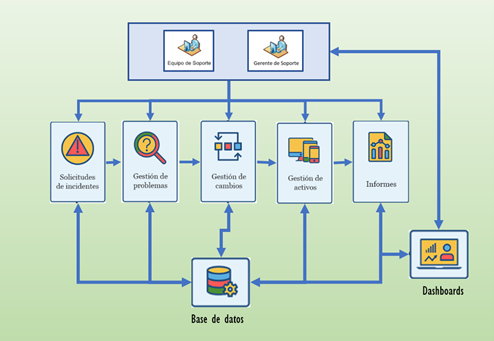
\includegraphics[width=0.9\textwidth]{Capitulo1/Img/MesadeServicioDiagrama}
	\caption{Arquitectura de mesa de servicio, como servicio}
	\label{fig:DMDS}
\end{figure}

\textbf{ Usuarios }

En el siguiente modulo se encuentran el usuario final, referidos como el Equipo de soporte y Gerente de soporte, los cuales tendrán la interacción con la interfaz de sistema con la finalidad de alimentar la base de datos, con los datos necesarios para la gestión correcta de los incidentes.\\

\textbf{Solicitudes de Incidencias }

En este módulo se gestiona y registra la información necesaria para el levantamiento de una solicitud de incidencia el cual dará comienzo al proceso del sistema de mesa de servicio.\\

\textbf{Gestión de problemas }

Durante esta etapa se analizará la información otorgada por el módulo 1.2 para conocer el tipo de incidencias y complejidad de solución y así asignar un nivel de atención.\\

 \textbf{Gestión de cambios.}
 
En este módulo después de un análisis realizado por el personal de soporte en sitio, se evaluará el nivel de atención, de acuerdo con la nueva información recabada y se realizaran los cambios necesarios si así lo amerita.\\

\textbf{Gestión de Activos }

Durante este módulo se realizarán las gestiones de Activos disponibles para poder atender las necesidades de las diversas incidencias.\\

\textbf{ Informes }

En este módulo se genera un medio de consulta diaria, con la finalidad de otorgar visibilidad de las condiciones operativas y administrativas de los incidentes.\\

\textbf{ Base de Datos }

Es el módulo encargado de almacenar, resguardar, organizar y facilitar la información, con el fin de gestionar las incidencias y proporcionar estadistas históricas de estas.

\subsection{Integración de mesa a la plataforma como servicio (PaaS)}


Se propone el desarrollo de un servicio web que integre cada uno de los requerimientos anteriores expuestos en el Figura \ref{fig:DMDS}. En la figura \ref{fig:AMDS} muestra la interacción entre los actores del sistema que, así como la comunicación entre ellos basada en protocolos de comunicación de internet, generando el sistema web de Mesa de Servicio desarrollado con las mejores prácticas.

\begin{figure}[htb]
	\centering
	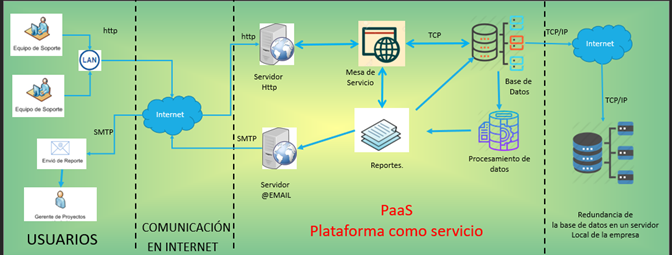
\includegraphics[width=0.9\textwidth]{Capitulo1/Img/AMDS}
	\caption{Intregacion de MS con la arquitectura del sistema como Infraesturura PaaS}
	\label{fig:AMDS}
\end{figure}

 \textbf{Usuarios}
 
Correspondiente al usuarios contendrá a todos los usuarios del sistema, estos realizasen una conexión al servicio web a través de internet con un Localizador Uniforme de Recursos (URL) del hosting que sea asignado al servicio haciendo estas conexiones bajo el protocoló de comunicación HTTP, así mismo tendrán la interacción directa con las interfaces del sistema, que contendrán las herramientas necesarias para la gestión de las atenciones de los servicios de incidencias brindadas por PyME. 
El modulo  usuarios de mesa de servicio se encargará de capturar e ingresar datos al sistema, con esta requisición se enviarán al servicio alojado en la nube.

\textbf{Nube plataforma como servicio (PaaS).}

El módulo  se contendrán al menos 3 subprocesos, alojados en la plataforma como servicio (PaaS) en de algún proveedor de nube ya sea AWS, GOOGLE CLOUD o bien AZURE 
\begin{itemize}

\item \textbf{“Servidor HTTP” }

 será el encargado procesar las solicitudes de conexión a nuestro servicio, así como denegar todas aquellas que no puedan identificarse así mismo todas las solicitudes serán procesadas bajo el protocolo http.
 
\item \textbf{“Mesa de Servicio” }

se encargará de alojar a todo el esquema de codificación del servicio web, estará basado tecnologías web, HTML, JAVA SCRIP Y CSS, este submódulo será el más importante, sus métodos de conexión serán hacia al servidor de Base de datos por el Protocolo TCP.
\item \textbf{“Procesamiento de datos” }
se encargará de llevar a cabo todo el procesamiento de datos contenidos en la base de datos con la finalidad brindar un reporteo de los datos ya mencionados, en este submódulo se implementarán todos los algoritmos de análisis, directamente relacionado con el módulo 1.6.

\item \textbf{“Base de Datos” }
Contendrá la base de Datos con base a un modelo relacional (Base de datos SQL), la interacción entre los módulos de procesamiento de datos y el submódulo de “Mesa de Servicio” se generarán con el protocolo TCP.
\textbf{“Reportes”}
 aunque es una función de los submódulos “procesamiento de información” y “base de datos”, se considera independiente en la arquitectura, por su importancia en el sistema, ya que esta contiene la información ya procesa y con un nivel de utilidad alto para la empresa, así mismo esta   será trasferida a  un submódulo consecuente que a su vez empaquetara y enviara baja el esquema de un correo electrónico, esta función será dirigida por el protocolo SMTP.

\item  \textbf{“Servidor Email”} se encargará de gestionar los correos electrónicos, el lugar donde se almacenan y la forma en la que se envían y reciben mensajes. Su principal función es la de enviar o recibir correos desde un host o servidor hacia distintos destinos a través de internet, la comunicación con internet se hará bajo el proto SMTP.

\end{itemize}


 \textbf{Redundancia de datos en un servidor local} 
 
El ultimo modulo llamado Redundancia de datos en un servidor local, se encargará de generar un respaldo solo de la base de datos del sistema ya que es prioritario tener una copia de seguridad de los datos en un servidor local que no dependa de la infraestructura de la nube, La infraestructura de la nube y en específico el gestor de base de datos harán una conexión con el servidor de la empresa ISAe, bajo los protocolos de comunicación TCP/IP.

\subsection{Integración con ERP}

La empresa PyME solicitante del desarrollo de la mesa de servicio, en la actualidad basa sus actividades en un esquema de ERP, sin embargo, carece de un carece de un servicio que le proporcione la administración, coordinación y gestión de los incidentes, al desarrollar el software como se menciona en los puntos anteriores se da una solución a esta necesidad, sin embargo para lograr tener un optimo desempeño de todo su sistema, la solución de  mesa de servicio será integrado al ERP, como se muestra en la figura \ref{fig:ERP-MDS} .
\begin{figure}[htb]
	\centering
	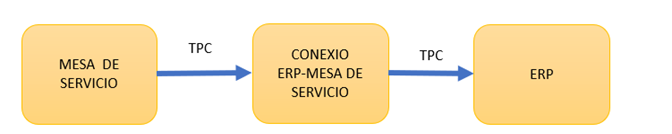
\includegraphics[width=0.9\textwidth]{Capitulo1/Img/ERP-MDS}
	\caption{Implementación de Mesa de Servicio en ERP}
	\label{fig:ERP-MDS}
	
\end{figure}


\textbf{Modulo mesa de servicio.}

El modulo  de  mesa de servicio representa el funcionamiento correcto de forma independiente como servicio y procesos, esta a su vez contara con toda la arquitectura ya antes mencionada en los figura \ref{fig:DMDS} y  la figura \ref{fig:AMDS}.

\textbf{Modulo de conexión }

En este módulo, estará alojada la conexión entre el ERP propiedad de la PyME así como Mesa de servicio desarrollada en esta investigación, esta modulo estará desarrollo con estructura de middleware, esta estará realizada bajo los protocolos de conexión de internet, como lo es TCP.

\textbf{Modulo ERP }

En este módulo se encuentra representada el ERP en el cual basa su funcionamiento la PyME.


\section{Alcances} 
De acuerdo con el desarrollo de solución propuesta se definen los siguientes alcances:
\begin{itemize}
\item Quedan excluidas las siguientes gestiones de la operación de servicio: gestión de acceso y 
gestión de eventos.

\item Quedan excluidas las siguientes disciplinas: estrategia del servicio, diseño del servicio, 
transición del servicio y mejora continua del servicio.

\item La mesa de servicio solo atenderá los  procesos establecidos para la atención, gestión y cierre  de incidencias por la PyME. 

\item Solo se incluirán los roles necesarios para el ciclo de vida de la atención de incidentes.

\item Se incluyen el uso solo de servidores necesarios para el despliegue de la solución propuesta. 

\item El modulo de Redundancia de Datos en un Servidor Local se gestionara solo en las bases de datos.

\item La integración de la mesa al ERP, solo se llevara acabo si el acuerdo de colaboración así lo permite, de no cumplirse, se excluirá de la solución propuesta.
\end{itemize}


\section{Objetivo General} 


Desarrollar una mesa de servicios para una PyME, basada en las mejores prácticas ITIL  e implementada en una plataforma como servicio (PaaS), que permita gestionar, coordinar y administrar incidentes. 


\section{Objetivos específicos} %Escribir al final
\begin{itemize}
	
\item Diseñar la mesa de servicios en base al proceso de desarrollo del catálogo de servicios  aplicando la gestión de niveles de servicio que permita mejorar los procesos de operación para  resolución de peticiones, incidentes y/o problemas.

\item Implementar la función de la mesa de servicios en base al catálogo diseñado, con los acuerdos 
de nivel de servicio y los procesos de operación del servicio establecidos para validar su 
correcto funcionamiento.

\item Desarrollar la mesa de servicio, como servicio web.

\item implementar el desarrollo de mesa de servicio en una plataforma de nube.
\end{itemize}



